\let\negmedspace\undefined
\let\negthickspace\undefined
%\RequirePackage{amsmath}
\documentclass[journal,12pt,twocolumn]{IEEEtran}
\usepackage[export]{adjustbox}
\usepackage{tabularx}
% \usepackage{setspace}
 \usepackage{gensymb}
%\doublespacing
%\singlespacing
%\usepackage{silence}
%Disable all warnings issued by latex starting with "You have..."
\usepackage{graphicx}
\usepackage{amssymb}
%\usepackage{relsize}
\usepackage[cmex10]{amsmath}
%\usepackage{amsthm}
%\interdisplaylinepenalty=2500
%\savesymbol{iint}
%\usepackage{txfonts}
%\restoresymbol{TXF}{iint}
%\usepackage{wasysym}
\usepackage{amsthm}
%\usepackage{iithtlc}
% \usepackage{mathrsfs}
% \usepackage{txfonts}
% \usepackage{stfloats}
% \usepackage{steinmetz}
 \usepackage{bm}
% \usepackage{cite}
% \usepackage{cases}
% \usepackage{subfig}
%\usepackage{xtab}
\usepackage{longtable}
%\usepackage{multirow}
%\usepackage{algorithm}
%\usepackage{algpseudocode}
\usepackage{enumitem}
 \usepackage{mathtools}
% \usepackage{tikz}
% \usepackage{circuitikz}
% \usepackage{verbatim}
%\usepackage{tfrupee}
\usepackage[breaklinks=true]{hyperref}
%\usepackage{stmaryrd}
%\usepackage{tkz-euclide} % loads  TikZ and tkz-base
%\usetkzobj{all}
\usepackage{listings}
    \usepackage{color}                                            %%
    \usepackage{array}                                            %%
    \usepackage{longtable}                                        %%
    \usepackage{calc}                                             %%
    \usepackage{multirow}                                         %%
    \usepackage{hhline}                                           %%
    \usepackage{ifthen}                                           %%
  %optionally (for landscape tables embedded in another document): %%
    \usepackage{lscape}     
 \usepackage{multicol}
% \usepackage{chngcntr}
%\usepackage{enumerate}

%\usepackage{wasysym}
%\newcounter{MYtempeqncnt}
\DeclareMathOperator*{\Res}{Res}
%\renewcommand{\baselinestretch}{2}
\renewcommand\thesection{\arabic{section}}
\renewcommand\thesubsection{\thesection.\arabic{subsection}}
\renewcommand\thesubsubsection{\thesubsection.\arabic{subsubsection}}

\renewcommand\thesectiondis{\arabic{section}}
\renewcommand\thesubsectiondis{\thesectiondis.\arabic{subsection}}
\renewcommand\thesubsubsectiondis{\thesubsectiondis.\arabic{subsubsection}}

% correct bad hyphenation here
\hyphenation{op-tical net-works semi-conduc-tor}
\def\inputGnumericTable{}                                 %%

\lstset{
%language=C,
frame=single, 
breaklines=true,
columns=fullflexible
}

\begin{document}
%

\newtheorem{theorem}{Theorem}[section]
\newtheorem{problem}{Problem}
\newtheorem{proposition}{Proposition}[section]
\newtheorem{lemma}{Lemma}[section]
\newtheorem{corollary}[theorem]{Corollary}
\newtheorem{example}{Example}[section]
\newtheorem{definition}[problem]{Definition}
%\newtheorem{thm}{Theorem}[section] 
%\newtheorem{defn}[thm]{Definition}
%\newtheorem{algorithm}{Algorithm}[section]
%\newtheorem{cor}{Corollary}
\newcommand{\BEQA}{\begin{eqnarray}}
\newcommand{\EEQA}{\end{eqnarray}}
\newcommand{\define}{\stackrel{\triangle}{=}}
\bibliographystyle{IEEEtran}
%\bibliographystyle{ieeetr}
\providecommand{\mbf}{\mathbf}
\providecommand{\pr}[1]{\ensuremath{\Pr\left(#1\right)}}
\providecommand{\qfunc}[1]{\ensuremath{Q\left(#1\right)}}
\providecommand{\sbrak}[1]{\ensuremath{{}\left[#1\right]}}
\providecommand{\lsbrak}[1]{\ensuremath{{}\left[#1\right.}}
\providecommand{\rsbrak}[1]{\ensuremath{{}\left.#1\right]}}
\providecommand{\brak}[1]{\ensuremath{\left(#1\right)}}
\providecommand{\lbrak}[1]{\ensuremath{\left(#1\right.}}
\providecommand{\rbrak}[1]{\ensuremath{\left.#1\right)}}
\providecommand{\cbrak}[1]{\ensuremath{\left\{#1\right\}}}
\providecommand{\lcbrak}[1]{\ensuremath{\left\{#1\right.}}
\providecommand{\rcbrak}[1]{\ensuremath{\left.#1\right\}}}
\theoremstyle{remark}
\newtheorem{rem}{Remark}
\newcommand{\sgn}{\mathop{\mathrm{sgn}}}
\providecommand{\abs}[1]{\left\vert#1\right\vert}
\providecommand{\res}[1]{\Res\displaylimits_{#1}} 
\providecommand{\norm}[1]{\left\lVert#1\right\rVert}
%\providecommand{\norm}[1]{\lVert#1\rVert}
\providecommand{\mtx}[1]{\mathbf{#1}}
\providecommand{\mean}[1]{E\left[ #1 \right]}
\providecommand{\fourier}{\overset{\mathcal{F}}{ \rightleftharpoons}}
%\providecommand{\hilbert}{\overset{\mathcal{H}}{ \rightleftharpoons}}
\providecommand{\system}{\overset{\mathcal{H}}{ \longleftrightarrow}}
  %\newcommand{\solution}[2]{\textbf{Solution:}{#1}}
\newcommand{\solution}{\noindent \textbf{Solution: }}
\newcommand{\cosec}{\,\text{cosec}\,}
\providecommand{\dec}[2]{\ensuremath{\overset{#1}{\underset{#2}{\gtrless}}}}
\newcommand{\myvec}[1]{\ensuremath{\begin{pmatrix}#1\end{pmatrix}}}
\newcommand{\mydet}[1]{\ensuremath{\begin{vmatrix}#1\end{vmatrix}}}
%\numberwithin{equation}{section}
\numberwithin{equation}{subsection}
%\numberwithin{problem}{section}
%\numberwithin{definition}{section}
\makeatletter
\@addtoreset{figure}{problem}
\makeatother
\let\StandardTheFigure\thefigure
\let\vec\mathbf
%\renewcommand{\thefigure}{\theproblem.\arabic{figure}}
\renewcommand{\thefigure}{\theproblem}
%\setlist[enumerate,1]{before=\renewcommand\theequation{\theenumi.\arabic{equation}}
%\counterwithin{equation}{enumi}
%\renewcommand{\theequation}{\arabic{subsection}.\arabic{equation}}
\def\putbox#1#2#3{\makebox[0in][l]{\makebox[#1][l]{}\raisebox{\baselineskip}[0in][0in]{\raisebox{#2}[0in][0in]{#3}}}}
     \def\rightbox#1{\makebox[0in][r]{#1}}
     \def\centbox#1{\makebox[0in]{#1}}
     \def\topbox#1{\raisebox{-\baselineskip}[0in][0in]{#1}}
     \def\midbox#1{\raisebox{-0.5\baselineskip}[0in][0in]{#1}}
\vspace{3cm}
\title{CBSE $10^{th}$ 2008 Question Paper}

\maketitle
\newpage
%\tableofcontents
\bigskip
\section{Section-A}
\renewcommand{\theequation}{\theenumi}
\begin{enumerate}
\item Complete the missing entries in the following factor tree :\\
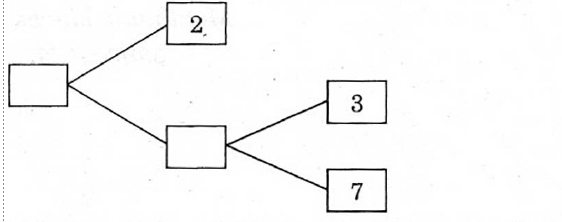
\includegraphics[width=\columnwidth, center]{1.png}
\label{fig:Line between A and B}
\item If (x + a) is a factor of 2x2 + 2ax + 5x + 10,find a.\\
\item  Show that x = - 3 is a solution of x2 + 6x + 9 = 0.\\
\item The first term of an A.P. is p and its common difference is q. Find its 10th term. \\
\item If tan A &= ($\frac{5}{12}$), find the value of (Sin A + Cos A)Sec A.\\
\item The lengths of the diagonals of a rhombus are 30 cm and 40 cm. Find the side of the rhombus. \\
\item In Figure 1, $PQ||BC$ and AP : PB = 1 : 2. Find ($\frac{ar(\Delta APQ}{ar(\Delta ABC}$).\\
{\centering
    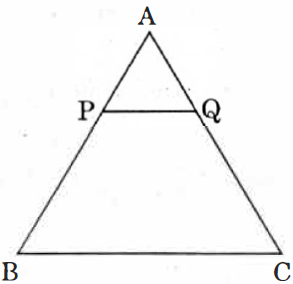
\includegraphics[width=5cm, center]{2.png}
    \caption{Figure 1 \\ }
    \label{Some label}}
\item The surface area of a sphere is 616 $cm^2$. Find its radius.\\
\item A die is thrown once. Find the probability of getting a number less than 3.\\  
\item Find the class marks of classes 10 -25 and 35 -55 . \\
\section{Section-B}
\item Find all the zeros of the polynomial $x^4+x^3-34x^2-4x=120$, if two of its zeros are 2,-2.\\
\item A pair of dice is thrown once. Find the probability of getting the same number on each dice. \\
\item If sec 4A = cosec (A - 20\textdegree), where 4A is an acute angle, find the value of A.
{\centering

    \caption{\textbf{\vec{OR}}\\ }
                        }
In a ,$\Delta$ ABC, right-angled at C, if tan A &= ($\frac{1}{\sqrt{3}}$) , find the value of
sin A cos B + cos A sin B.
\item Find the value of k if the points (k, 3), (6, -2) and {-3, 4) are collinear.\\
\item E is a point on the side AD produced of a $||^{gm}$ ABCD and BE intersects CD at F. Show that $\Delta$ ABE \sim $\Delta$ CFB.
\section{Section-C}
\item Use Euclid's Division Lemma to show that the square of any positive integer is either of the form 3m or (3m + 1) for some integer m.\\ 
\item Represent the following pair of equations graphically and write the coordinates of pointswhere the lines intersect y-axis:\\
$x+3y=6$ \\
$2x-3y=12$ \\
\item For what value of n are the $n^{th}$ terms of two A.P.'s 63, 65, 67, ... and 3, 10, 17, ... equal ?\\
{\centering

    \caption{\textbf{\vec{OR}}\\ }
                        }
If m times the $m^{th}$ term of an A.P. is equal to n times its $n^{th}$ term, find the $(m+n)^{th}$ term of the A.P.
\item In an A,P., the first term is 8, $n^{th}$ term is 33 and sum to first n terms is 123. Find n and d, the common difference.\\
\item Prove that :
(1 + cotA+ tanA) (sinA - cosA)= sinA tanA - cotA cosA.\\
{\centering

    \caption{\textbf{\vec{OR}}\\ }
                        }
Without using trigonometric tables, evaluate the following:\\
2 $\frac{cos58\degree }{sin32\degree} - \sqrt{3}\frac{cos38\degree cosec52\degree}{tan15\degree tan60\degree tan75\degree}$\\
\item If P divides the join of A(-2, -2) and B(2, -4) such that $\frac{AP}{AB}$ &= $\frac{3}{7}$, find the coordinates of P.\\
\item The mid-points of the sides of a triangle are (3, 4), (4, 6) and (5, 7). Find the coordinates· of the vertices of the triangle.\\
\item Draw a right triangle in which the sides containing the right angle are 5 cm and 4 cm. Construct a similar triangle whose sides are. $\frac{5}{3}$ times the sides of the above triangle.\\
\item Prove that a parallelogram circumscribing a circle is a rhombus.

{\centering

    \caption{\textbf{\vec{OR}}\\ }
                        }
In Figure 2, AD $\perp$ BC. Prove that $AB^2 + CO^2 = B0^2 + AC^2$.
{\centering
    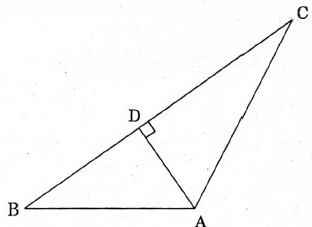
\includegraphics[width=5cm, center]{4.png}
    \caption{Figure 2 \\ }
    \label{Some label}}
\item In Figure 3, ABC is a quadrant of a circle of radius 14 cm and a semi-circle is drawn with BC as diameter. Find the area of the shaded region.

{\centering
    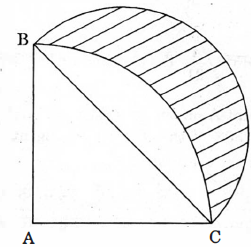
\includegraphics[width=5cm, center]{5.png}
    \caption{Figure 3 \\ }
    \label{Some label}}
    
\section{Section-D}

\item A peacock is sitting on the top of a pillar, which is 9 m high. From a point 27 m away from the bottom of the pillar, a snake is coming to its hole at the base of the pillar. Seeing the sn'ake the peacock pounces on it. If their speeds are equal, at what distance from the hole is the snake caught ?\\
{\centering

    \caption{\textbf{\vec{OR}}\\ }
                        }
The difference of two numbers is 4. If the difference of their reciprocals $\frac{4}{21}$  is , find the two numbers. \\
\item The angle of elevation of an aeroplane from a point A on the ground is 60\textdegree. After a flight of 30 seconds, the angle of elevation changes to 30\textdegree. If the plane is flying at a constant
height of 3600 $\sqrt{3}$ m, find the speed, in km/hour, of the plane .\\
\item If a line is drawn parallel to one side of a triangle to intersect the other two sides in distinct points, prove that the other two sides are divided in the same ratio.\\
Using the above, prove the following :\\
In figure 4, $AB\parallel DE$ and $BC \parallel EF$. Prove that $AC \parallel DF$.

{\centering
    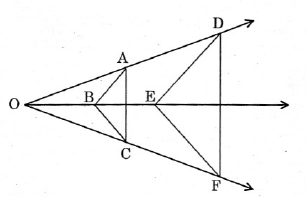
\includegraphics[width=5cm, center]{6.png}
    \caption{Figure 4 \\ }
    \label{Some label}}

{\centering

    \caption{\textbf{\vec{OR}}\\ }
                        }

Prove that the lengths of tangents drawn from an external point to a circle are equal. Using the above, prove the following : \\
ABC is an isosceles triangle in which AB = AC, circumscribed about a circle, as shown in Figure 5. Prove that the base is bisected by the point of contact. \\

{\centering
    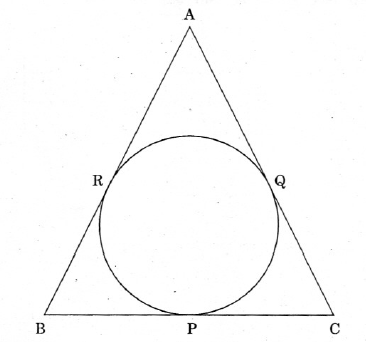
\includegraphics[width=5cm, center]{7.png}
    \caption{Figure 5 \\ }
    \label{Some label}}

\item If the radii of the circular ends of a conical bucket, which is 16 cm high, are 20 cm and 8 cm, find the capacity and total surface area of the bucket. [Use $\pi$ &= $\frac{22}{7}$ ]\\
\item Find mean, median and mode of the following data :\\

\begin{tabularx}{\columnwidth} { 
  | >{\centering\arraybackslash}X 
  | >{\centering\arraybackslash}X | }
 \hline
 Class & Frequency  \\
 \hline
 0-20  &  6   \\
\hline
  20-40 &  8  \\
 \hline
 40-60  &  10   \\
\hline
 60-80 &  12  \\
 \hline
 80-100  &  6   \\
\hline
100-120 &  5  \\
 \hline
 120-140  &  3   \\
\hline
\end{tabularx}
\end{enumerate}
\end{document}
